\begin{frame}{Stødende jagthunde}

\vspace{1em}

\begin{columns}[c] % c = center vertically

\column{0.05\textwidth} % Venstre margin

\column{0.7\textwidth} % Midten: Bullets

\small

\raggedright

\begin{itemize}

\itemsep0.6em % Justér afstand mellem bullets

\item Hundens opgave er at \textbf{søge under bøssen} (tæt på jægeren) og rejse vildtet.
\item De skal "støde" vildtet, dvs. få det til at \textbf{flyve eller løbe op} inden for skudafstand.
\item Har typisk en \textbf{kort rækkevidde} i søget og arbejder tæt sammen med jægeren.
\item Bruges primært til jagt på \textbf{fugle} (f.eks. fasaner og ænder) og \textbf{kaniner}.
\item \textbf{Racer}: Cocker Spaniel, Springer Spaniel, Field Spaniel, Kleiner Münsterländer (kan også stå).

\end{itemize}

\column{0.25\textwidth} % Højre: Ikon

\centering

\vspace{0pt}

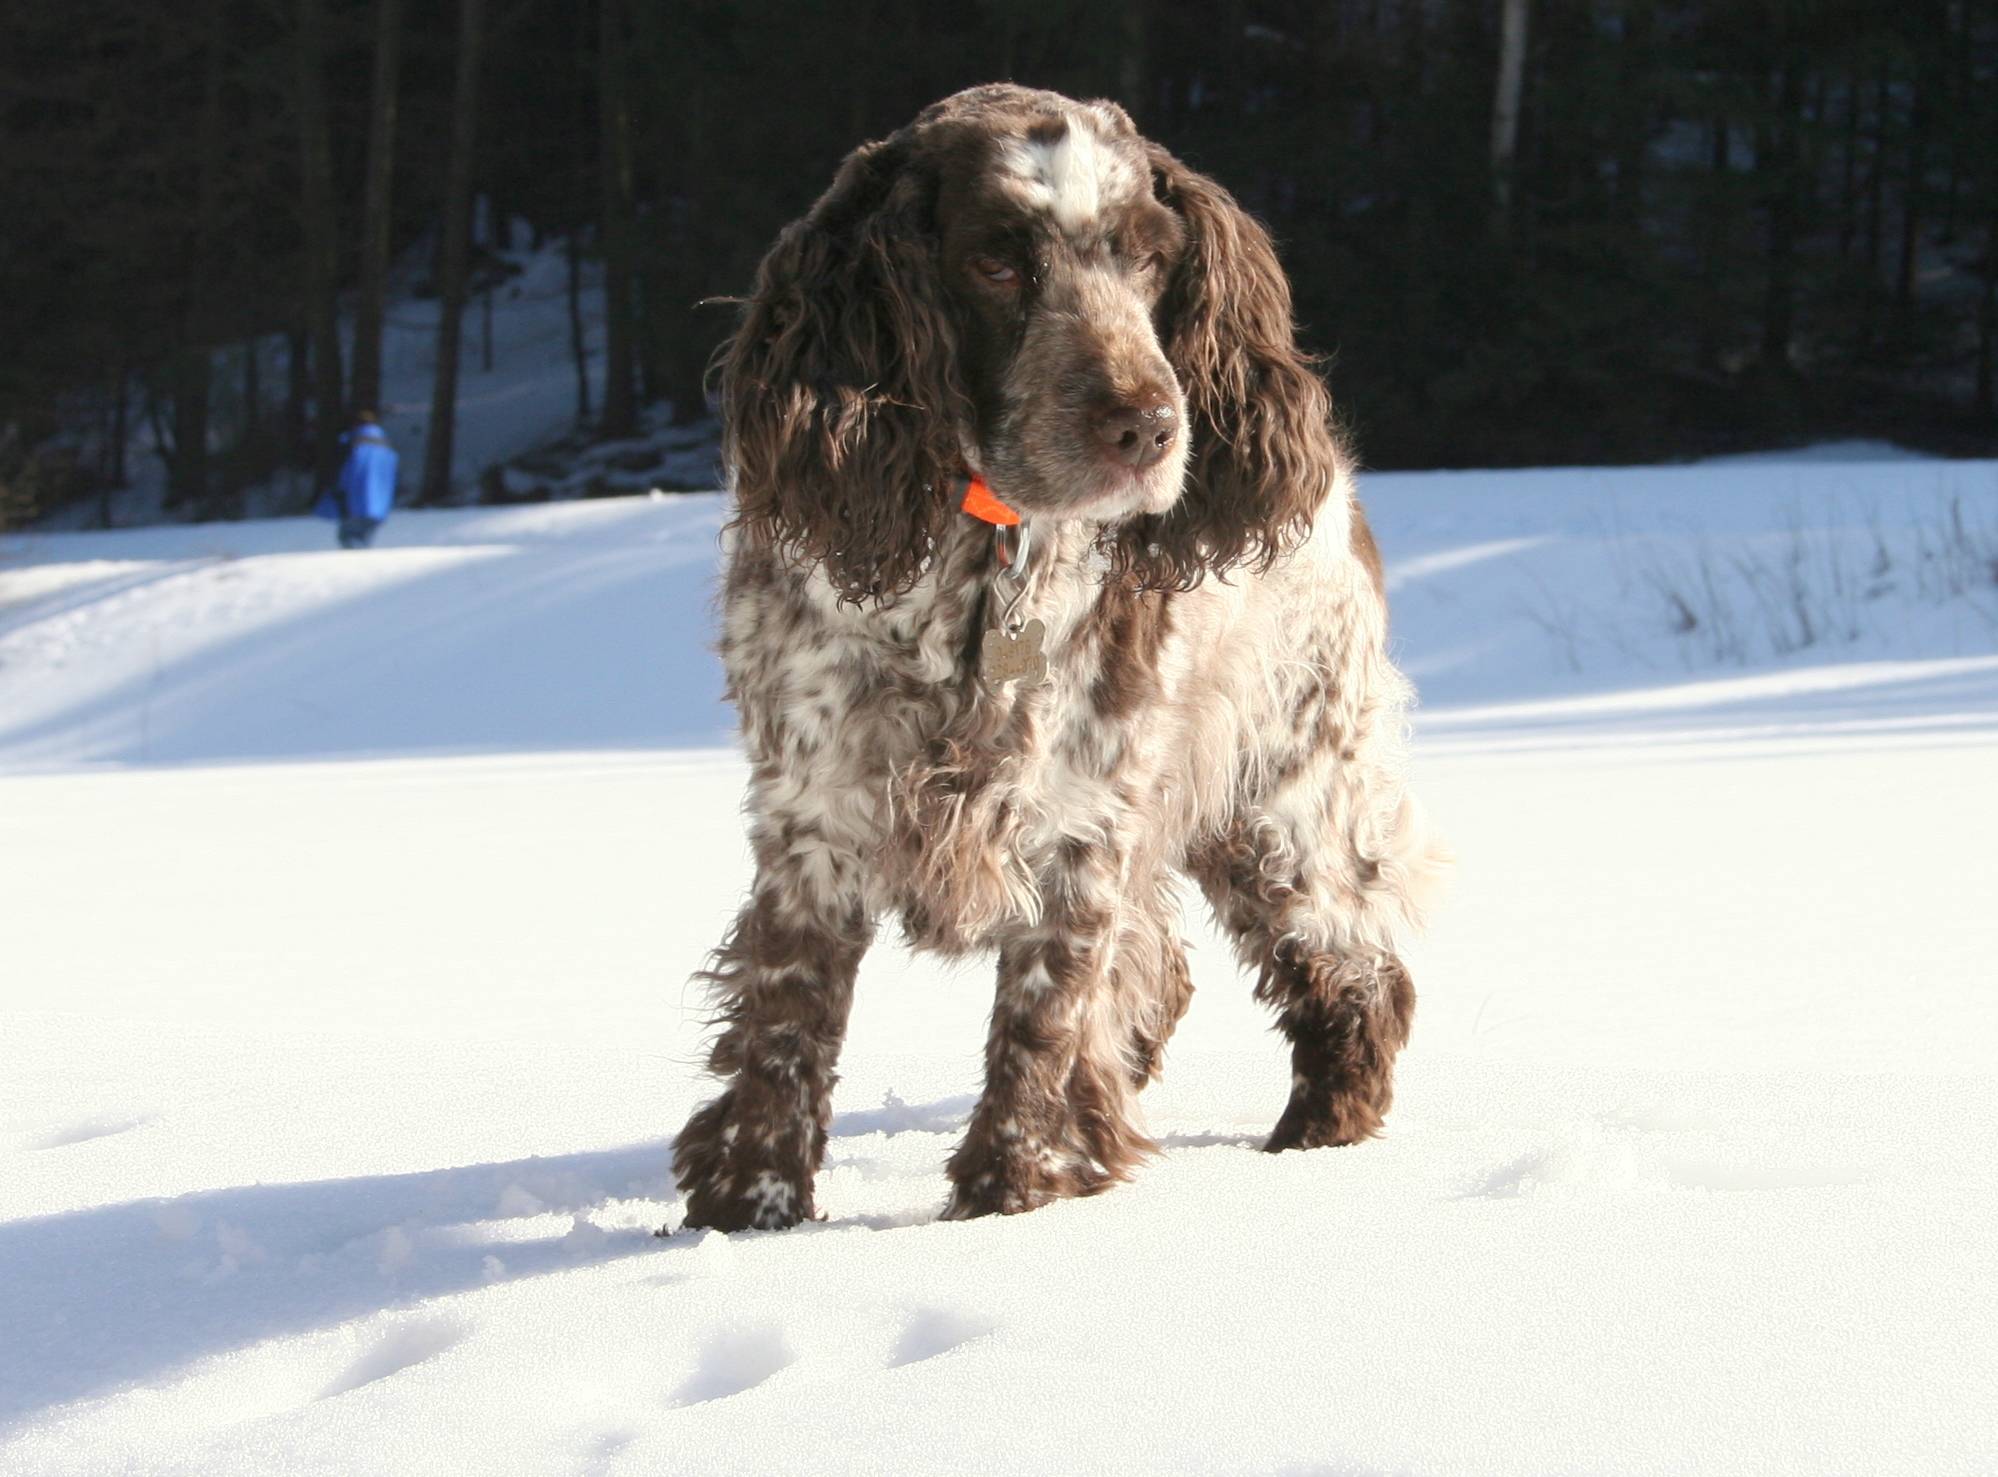
\includegraphics[width=0.9\linewidth]{Billeder/Jagthunde/stoedende/cocker.jpg} % Ikon af en spaniel i aktion

\end{columns}

\end{frame}